\section{Research II-C -- Causal Prediction, Replay Retention, and Real-Runtime Validation}
\label{sec:iic}

Research~II-C evaluates whether a strictly causal predictor can exploit the
routing structure characterized in Research~II-B, whether a predictor-driven
retention policy built on it improves a replay-level retention metric, and
whether that replay-level improvement converts into measured real-runtime
decode-throughput improvement. We preserve throughout this section the
three-level distinction stated in the programme's original roadmap
(Section~\ref{sec:introduction}'s enumeration of II-A/II-B/II-C, and
Section~\ref{sec:recoverable-envelope}'s unmeasured-comparator-relative
discussion, both retained unchanged): \emph{prediction} (R2-09/R2-10),
\emph{replay-level retention} (R2-BRIDGE-01/R2-11), and \emph{real runtime}
(R2-12) are three separate, differently-scoped measurements. A result at one level does not imply, and
is not treated here as implying, the same result at another level.

\begin{table}[t]
\centering
\caption{Causal-prediction and real-runtime-validation milestone summary.}
\label{tab:c1-milestones}
\small
\begin{tabular}{@{}lp{6.3cm}l@{}}
\toprule
Milestone & Purpose & Closure state \\
\midrule
R-09A/B & Freeze benchmark contract; DEV causal-baseline tournament & CLOSED \\
R-10 & Held-out EVAL of selected predictor (decayed\_transition) & CLOSED / Category B supported \\
R-BRIDGE-01 & Prospective replay retention feasibility check & CLOSED / BRIDGE\_POSITIVE \\
R-11 & Confirmatory replay retention evaluation, 72 cells & CLOSED / R2\_11\_PASS \\
R-12 & Real-runtime validation, 1.5/4/8 GiB & CLOSED / R2\_12\_FAIL (primary) \\
\bottomrule
\end{tabular}
\end{table}


\subsection{R2-09/R2-10 -- Causal Working-Set Prediction}
\label{sec:r2-10}

Under the frozen R2-09B benchmark contract (DEV/EVAL role separation,
leakage-safe baseline selection, deterministic double-scoring), the DEV
causal-baseline tournament selected \texttt{decayed\_transition} (decay
$=0.99$) as the best-performing causal predictor family on 8 DEV cells,
with DEV $h=1$ mean recall$@k$ $0.439397$ against the best trivial causal
baseline (\texttt{last\_observation}, $0.406808$), an absolute margin of
$0.032589$. Under \texttt{decision\_rules.json}'s DEV-anchored category
definitions this margin is classified Category~B
(\textsc{measurable\_improvement\_insufficient\_for\_retention}): measurable
and consistent across all 8 DEV cells and all 4 workload families, but not
large enough to meet the Category~C bar on its own.

On 4 sealed, held-out EVAL instances (captured and sealed before scoring),
the selected predictor's $h=1$ mean recall$@k$ was $0.449817$, exceeding its
own DEV figure (no sign of DEV overfitting), and beating both trivial
baselines: \texttt{last\_observation} ($0.401473$, $+12.04\%$ relative) and
\texttt{global\_frequency} ($0.349480$, $+28.71\%$ relative). The margin over
\texttt{last\_observation} was positive in all 4 workloads at every tested
horizon ($h=1,4,16$); the margin over \texttt{global\_frequency} was positive
in all 4 workloads at $h=1$ and $h=4$ but negative in one workload
(instruction-eval-v1) at $h=16$, which we report as a disclosed negative
finding rather than omit. Because \texttt{decision\_rules.json}'s Category
A/B/C criteria are textually anchored to the DEV corpus, this held-out
evidence \emph{supports, without promoting}, the DEV-based Category~B
classification: EVAL data cannot itself satisfy a category defined only over
DEV cells. R2-09/R2-10 therefore establish a measurable, held-out-confirmed
causal prediction margin over trivial baselines, at a magnitude the frozen
rules themselves judge insufficient, standing alone, to justify retention
integration.

\begin{table}[t]
\centering
\caption{R2-09/R2-10 held-out EVAL mean recall@k by horizon (4 held-out instances, equal weight).}
\label{tab:c2-predictor}
\small
\begin{tabular}{@{}lccc@{}}
\toprule
Predictor & $h{=}1$ & $h{=}4$ & $h{=}16$ \\
\midrule
decayed\_transition (selected) & 0.4498 & 0.3611 & 0.3403 \\
last\_observation & 0.4015 & 0.2995 & 0.2648 \\
global\_frequency & 0.3495 & 0.3429 & 0.3322 \\
\bottomrule
\end{tabular}
\end{table}


\begin{figure}[t]
\centering
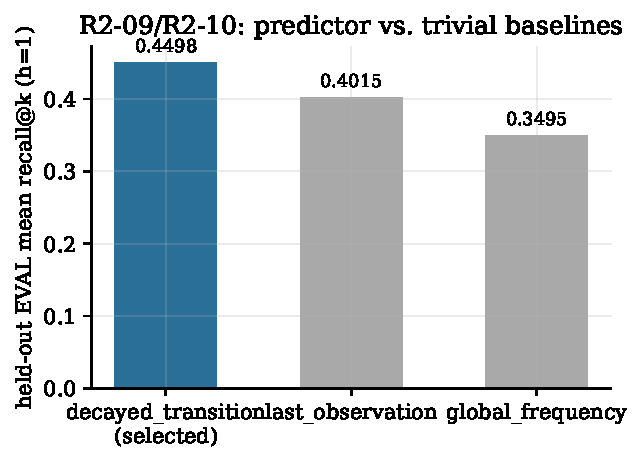
\includegraphics[width=0.68\linewidth]{figures/figure_c1_r2_10_predictor_comparison.pdf}
\caption{R2-09/R2-10: held-out EVAL mean recall@k ($h{=}1$) for the
selected predictor vs.\ both trivial causal baselines. Values read from
Table~\ref{tab:c2-predictor}.}
\label{fig:c1-predictor}
\end{figure}

\subsection{R2-BRIDGE-01 -- Retention Feasibility Bridge}
\label{sec:bridge01}

The literal historical statement that \emph{``R2-11 was NOT PROPOSED under
the original frozen R2-10 decision rules''} remains true and unchanged: the
Category~B finding above does not, by the original rule's own text, provide
a path to proposing a retention-integration experiment. R2-BRIDGE-01 is a
separate, later-frozen, prospective protocol -- not a retroactive
reinterpretation of R2-10's rule -- whose purpose was precisely to determine
whether \emph{new} evidence could justify proposing such an experiment.

Under a frozen contract and a DEV-selection rule fixed before held-out
capture, R2-BRIDGE-01 wired the selected R2-10 predictor into a reactive
retention policy, \texttt{PredictedProtectPolicy}, and compared it against
the aged-frequency baseline \texttt{B\_selected(M)} on 4 fresh held-out
instances, using \texttt{miss\_bytes\_per\_decode\_step} in replay. At the
primary 4~GiB budget, \texttt{PredictedProtect} reduced mean miss bytes per
decode step by $57{,}784.861$ (relative $-0.023084\%$) relative to
\texttt{B\_selected(M)}, with every one of the 4 held-out workloads
individually non-positive. At the two secondary budgets tested, the effect
was also non-positive (1.5~GiB: $-0.1335\%$; 8~GiB: exactly $0.0\%$, an exact
tie). R2-BRIDGE-01 was classified \textsc{bridge\_positive}: the effect is
small in absolute terms, but it is consistently signed across all tested
workloads and budgets, and that consistency -- not its magnitude -- is what
the frozen rule treats as sufficient to justify \emph{proposing} a new,
separate R2-11 protocol prospectively. This does not rewrite, and is not
read here as rewriting, the historical R2-10-rule statement above; both
statements hold simultaneously. No runtime-speedup claim is made or implied
by R2-BRIDGE-01: the metric is a replay-level memory-traffic proxy, not a
timing measurement.

\begin{figure}[t]
\centering
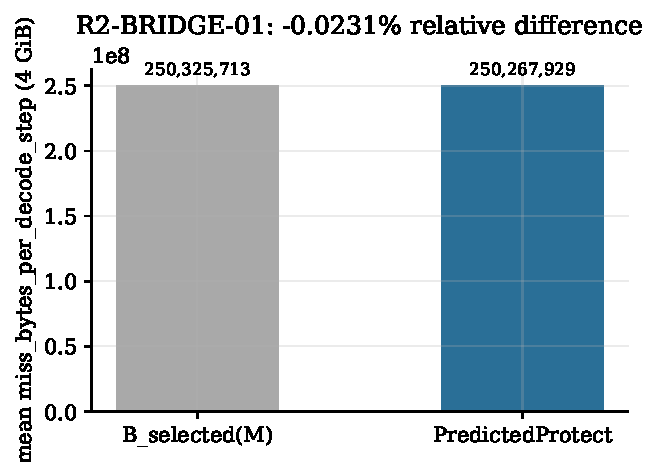
\includegraphics[width=0.6\linewidth]{figures/figure_c2_r2_bridge01_miss_bytes.pdf}
\caption{R2-BRIDGE-01: mean miss\_bytes\_per\_decode\_step, B\_selected(M)
vs.\ PredictedProtect, primary 4~GiB budget, 4 held-out instances.}
\label{fig:c2-bridge}
\end{figure}

\subsection{R2-11 -- Confirmatory Replay-Level Retention Evaluation}
\label{sec:r2-11}

R2-11 is the confirmatory evaluation proposed on the strength of
R2-BRIDGE-01's prospective result, run under its own frozen Phase-0 protocol
(fixed before any capture). It compares \texttt{PredictedProtect} against
\texttt{B\_selected(M)} on 12 fresh workload instances $\times$ 3 budgets
(1.5/4/8~GiB) $\times$ 2 policies, a $72$-cell design; all 72 cells were
computed, with 0 failures and 0 budget-constraint violations across the
full design.

At the frozen primary 4~GiB budget, the mean paired delta in
\texttt{miss\_bytes\_per\_decode\_step} was $-87{,}476.85$
(\texttt{PredictedProtect} minus \texttt{B\_selected(M)}), with a paired
bootstrap 95\% confidence interval of $[-154{,}123.32,\,-27{,}178.93]$ (100{,}000
resamples, fixed seed, independently audited for determinism) --
entirely below zero. 9 of the 12 workload instances individually improved
($\le 0$). At the 1.5~GiB stress budget the effect was larger in magnitude
($-779{,}296.06$); at the 8~GiB budget the effect was an exact tie
($0.0$ for all 12 workload instances), consistent with the budget being
generous enough, on these workloads, that eviction pressure -- and hence any
opportunity for a predictive eviction policy to change which object is
evicted -- is minimal or absent. R2-11's frozen decision rule classifies
this primary-budget result \textsc{r2\_11\_pass}.

We state explicitly, as the programme's evidence-level distinction requires:
\textsc{r2\_11\_pass} is a statement about
\texttt{miss\_bytes\_per\_decode\_step} under offline replay. It is
\emph{not} a runtime, latency, or throughput measurement, and it does not by
itself establish that any real decode-time benefit follows. That question is
R2-12's.

\begin{table}[t]
\centering
\caption{Replay-level retention results: mean paired delta in miss\_bytes\_per\_decode\_step (PredictedProtect $-$ B\_selected(M)).}
\label{tab:c3-retention}
\small
\begin{tabular}{@{}llrrrl@{}}
\toprule
Stage & Budget & $\Delta$ (bytes/step) & Relative & 95\% CI & Status \\
\midrule
R2-BRIDGE-01 (prospective) & 4 GiB (primary) & -57,784.86 & -0.0231\% & --- & BRIDGE\_POSITIVE \\
R2-11 (confirmatory) & 1.5 GiB (stress) & -779,296.06 & --- & --- & descriptive \\
R2-11 (confirmatory) & 4 GiB (primary) & -87,476.85 & --- & [-154,123.32, -27,178.93] & R2\_11\_PASS \\
R2-11 (confirmatory) & 8 GiB (null-control) & 0.00 & 0.0000\% & --- & exact tie \\
\bottomrule
\end{tabular}
\end{table}


\begin{figure}[t]
\centering
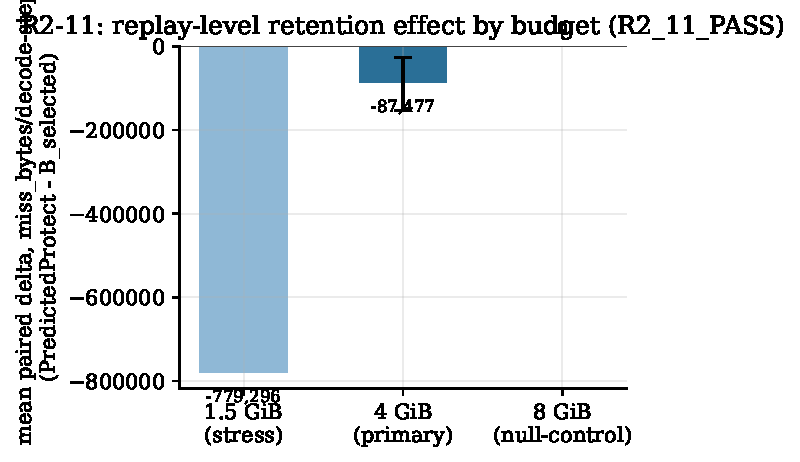
\includegraphics[width=0.78\linewidth]{figures/figure_c3_r2_11_replay_effect.pdf}
\caption{R2-11: mean paired delta in miss\_bytes\_per\_decode\_step by
budget (PredictedProtect $-$ B\_selected(M)); error bar shows the frozen
primary-budget 95\% paired bootstrap CI. 1.5/8~GiB are shown for context
and do not carry an independent R2-12-style classification at this stage.}
\label{fig:c3-r2-11}
\end{figure}

\subsection{R2-12 -- Real-Runtime Validation}
\label{sec:r2-12}

R2-12 tests whether R2-11's replay-level retention improvement converts into
measured real-runtime decode-throughput improvement, using the actual
30B-class runtime (not offline replay), under a frozen Phase-0 protocol with
machine-state and readiness gates fixed before any canonical acquisition.
Realizing the retention-policy integration in the real runtime required
several iterations before reaching an accepted conformance state (the
runtime binary used here is not byte-identical to the R2-01 validated
replay-comparison runtime; conformance was reached only after repeated
realization/repair cycles, not on the first attempt -- see
Section~\ref{sec:iic-limitations}). The frozen primary endpoint is the
4~GiB budget; 1.5~GiB (``stress'') and 8~GiB (``null-control'') are
secondary, descriptive budgets that cannot override the primary
classification under the frozen decision rule.

Across all three budgets, $144/144$ physical canonical launches were
completed (48 each at 1.5/4/8~GiB; 40 counted and 8 warmup per budget),
with all per-budget output-equivalence and integrity checks passing and the
frozen contract digest unchanged throughout. One latent software defect was
found and fixed mid-campaign -- the primary-analysis loader lacked a
budget-scoping filter, which was harmless until multiple budgets' canonical
records coexisted on disk -- and is disclosed here rather than silently
corrected; its fix is covered by a dedicated mixed-budget contamination
regression test, and the previously-committed 4~GiB result was verified
byte-identical before and after the fix.

At the \textbf{primary 4~GiB budget}, the observed mean paired delta in
decode tokens-per-second was $\mathbf{-0.171721}$
(\texttt{PredictedProtect} minus \texttt{B\_selected(M)}), 95\% paired
bootstrap CI $[-0.259917,\,-0.091642]$, entirely at or below zero;
\texttt{B\_selected(M)} won 18 of 20 counted pairs. Per the frozen primary
decision rule, this is sufficient on its own for a negative classification;
the separate overhead-dominance clause need not be evaluated. \textbf{R2-12's
primary classification is \textsc{r2\_12\_fail}.}

At the \textbf{1.5~GiB stress budget} (descriptive only, no independent
classification), the observed delta was $-0.068831$ TPS ($-2.9238\%$), 95\%
CI $[-0.093256,\,-0.054608]$. At the \textbf{8~GiB null-control budget}
(descriptive only), the observed delta was $-0.4373259$ TPS ($-6.5166\%$),
95\% CI $[-0.531584,\,-0.366601]$, with \texttt{B\_selected(M)} winning all
20 counted pairs. R2-11 found an exact replay-level retention tie at
8~GiB; R2-12 does not assume runtime equality follows from that tie, and
treats 8~GiB as a useful null/control condition in exactly this sense: a
material real-runtime difference despite (replay-level) retention-traffic
parity would, if it could be attributed to a specific mechanism, point away
from retention and toward some other overhead source. However, the real
8~GiB canonical records carry \emph{no} retention-traffic telemetry for
either policy at this budget (\texttt{expert\_bytes\_read},
\texttt{expert\_read\_count}, \texttt{expert\_miss\_bytes}, and every
\texttt{expert\_io\_best\_effort} sub-field are \texttt{None} in the real
acquisition for both policies). Consequently, any explanation of the 8~GiB
delta in terms of non-retention (e.g., prediction-policy bookkeeping)
overhead remains an explicitly unverified \emph{hypothesis}, not a
finding, in this manuscript.

Descriptively, the magnitude of the measured delta is smallest at 1.5~GiB
($-2.92\%$), intermediate at 4~GiB ($-4.77\%$), and largest at 8~GiB
($-6.52\%$). We state this as an \emph{observation over three tested
points}, not as evidence of a monotonic causal relationship between memory
budget and policy overhead, a claim the available design cannot support
with only three budget points and no isolated overhead mechanism.

\begin{table}[t]
\centering
\caption{R2-12 real-runtime results: mean paired delta in decode tokens/second (PredictedProtect $-$ B\_selected(M)), own 95\% CI per budget (not pooled).}
\label{tab:c4-runtime}
\small
\begin{tabular}{@{}lrll@{}}
\toprule
Budget & $\Delta$ TPS & 95\% CI & Classification \\
\midrule
1.5 GiB (stress) & -0.068831 & [-0.093256, -0.054608] & descriptive only \\
4 GiB (primary) & -0.171721 & [-0.259917, -0.091642] & R2\_12\_FAIL \\
8 GiB (null-control) & -0.437326 & [-0.531584, -0.366601] & descriptive only \\
\bottomrule
\end{tabular}
\vspace{2pt}
\par\footnotesize\textsuperscript{1}Secondary budgets are descriptive only and cannot override the primary 4~GiB classification under the frozen decision rule.
\end{table}


\begin{figure}[t]
\centering
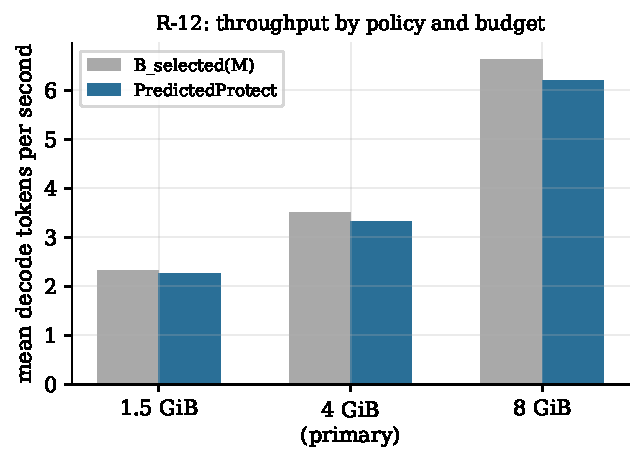
\includegraphics[width=0.78\linewidth]{figures/figure_c4_r2_12_throughput_by_budget.pdf}
\caption{R2-12: mean real-runtime decode tokens/second by policy and
budget. 4~GiB is the frozen primary endpoint; 1.5/8~GiB are secondary and
descriptive only.}
\label{fig:c4-r2-12-throughput}
\end{figure}

\begin{figure}[t]
\centering
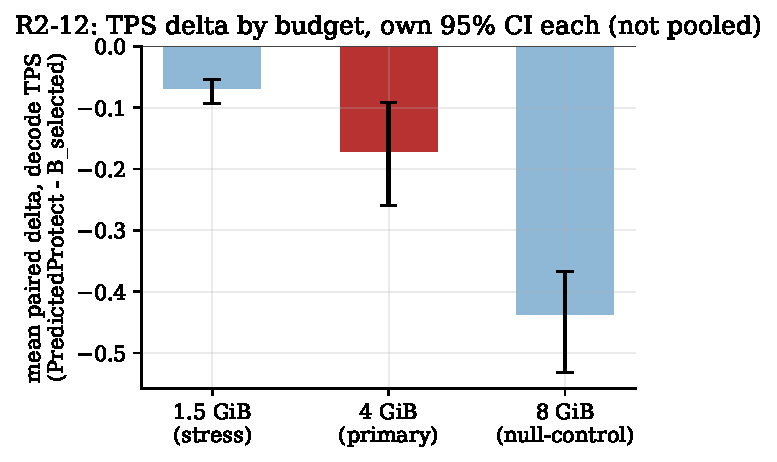
\includegraphics[width=0.78\linewidth]{figures/figure_c5_r2_12_delta_by_budget_ci.pdf}
\caption{R2-12: mean paired delta in decode tokens/second
(PredictedProtect $-$ B\_selected(M)) by budget, each with its own frozen
95\% paired bootstrap CI (not pooled across budgets). The primary 4~GiB
classification is \textsc{R2\_12\_FAIL}; 1.5/8~GiB are descriptive only and
do not carry an independent classification.}
\label{fig:c5-r2-12-delta}
\end{figure}

\subsection{Cross-Stage Synthesis}
\label{sec:iic-synthesis}

\begin{figure}[t]
\centering
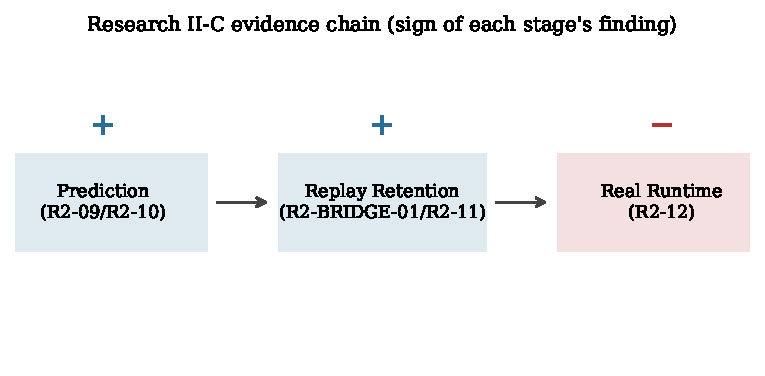
\includegraphics[width=0.78\linewidth]{figures/figure_c6_evidence_chain.pdf}
\caption{Research II-C evidence chain: prediction (positive) $\rightarrow$
replay retention (positive) $\rightarrow$ real runtime (negative). Each
stage measures a different quantity under a different experimental
apparatus; a negative result at one stage does not retroactively alter a
positive result at an earlier stage.}
\label{fig:c6-evidence-chain}
\end{figure}

\begin{center}
\begin{tabular}{@{}lll@{}}
\toprule
Level & Finding & Scope \\
\midrule
1. Prediction (R2-09/R2-10) & Positive (Category B; EVAL-confirmed margin) & Prediction quality only \\
2. Replay retention (R2-BRIDGE-01/R2-11) & Positive (\textsc{bridge\_positive}; \textsc{r2\_11\_pass}) & Replay miss-byte metric only \\
3. Real runtime (R2-12) & Negative (\textsc{r2\_12\_fail}) & Real decode throughput, primary budget \\
\bottomrule
\end{tabular}
\end{center}

These three findings are not in tension with one another: each measures a
different quantity, under a different (and progressively more realistic)
experimental apparatus, and none of the first two findings is invalidated by
the third. No predictor-quality or retention-improvement claim from R2-10,
R2-BRIDGE-01, or R2-11 is weakened, retracted, or reclassified merely
because real-runtime throughput failed to improve at R2-12.

The central conclusion of Research~II-C is accordingly conservative:
predictive expert information is measurably useful for forecasting routing
and can improve a replay-level retention metric, but the tested
\emph{reactive} predictive-retention realization -- one that only changes
which resident object is evicted on a miss, without changing when a fetch is
issued relative to ongoing computation -- does not convert that information
into improved end-to-end decode throughput on the evaluated runtime
configuration. Section~\ref{sec:iic-related-work} below situates this
result against systems in the literature that \emph{do} report throughput
gains from predictive expert handling.

\subsection{Related Work in Context}
\label{sec:iic-related-work}

A line of systems work on memory-constrained MoE inference reports measured
throughput or latency gains from combining expert-use prediction with an
\emph{active} mechanism for acting on that prediction before a miss reaches
the decode critical path: proactive prefetching with reordered inference
\cite{promoe2025}, joint prediction-plus-scheduling that explicitly
decouples I/O from computation \cite{prescope2025}, semantic-hint-driven
joint prefetch/cache/offload decisions \cite{finemoe2026}, predictive
caching paired with token scheduling \cite{expertflow2026}, data-aware
GPU-CPU hybrid prefetch/pre-calculation \cite{daop2025}, and speculative
pre-execution of likely-needed experts \cite{speculatingexperts2026}
(evaluated on the same Qwen3-30B-A3B model family used here)
\cite{moespeq2026}. Edge0 \cite{edge02026}, targeting the same
consumer-hardware, SSD-served deployment regime as this programme, predicts
the \emph{next} layer's routing one token ahead and stages the read during
the \emph{current} layer's computation, directly addressing the timing
constraint that a layer's expert set cannot be known before the previous
layer's output exists. Whether a given MoE model's routing is even
amenable to this class of techniques is itself an open question
\cite{localroutingconsistency2025}.

Every one of these systems pairs prediction with a mechanism that changes
\emph{when} a fetch is issued relative to compute. This programme's R2-12
realization tested only the narrower mechanism of changing \emph{which}
resident object is evicted on a reactive miss (\texttt{PredictedProtectPolicy}),
with no prefetch, scheduling, or compute/I/O overlap component. R2-12's
negative real-runtime result is consistent with this literature's implicit
premise -- that an active timing mechanism, not prediction alone, is what
converts predictive accuracy into measured throughput -- rather than being in
tension with it. This framing was available independent of, and is not a
retrofit to accommodate, the R2-12 outcome: the distinction between
retention (what is evicted) and prefetch/scheduling (when a fetch is issued)
is a property of the system designs being surveyed, not of Argine's result.
This programme does not claim priority or comparative superiority over any
of the cited systems; none was reimplemented or benchmarked head-to-head
against Argine's runtime.
